\documentclass[10pt]{beamer}
\usetheme{jambro}

\title[]{Macroeconomia I - Modelo IS-LM}
\author[]{\href{https://pvfonseca.github.io}{Paulo Victor da Fonseca}}
\date{}

\hypersetup{
    colorlinks = true,
    urlcolor = teal,
    linkcolor = teal    
}
\usepackage[portuguese]{babel}
\usepackage{subfig}
\usepackage{emoji}
\usepackage{hyperref}

\begin{document}

\begin{frame}[plain]
    \titlepage{
        \begin{center}
            \begin{minipage}{0.8\textwidth}
                \centering
            \end{minipage}
        \end{center}}
\end{frame}

\begin{frame}{Sumário}
    \tableofcontents
\end{frame}

\section{Teoria Keynesiana da taxa de juros}
\subsection{Introdução}
\begin{frame}{Introdução}
    \begin{itemize}
        \item Examinaremos, agora, a relação entre quantidade de moeda e taxa de juros.
        \bigskip
        \item O modelo clássico continha um papel para a moeda e a política monetária.
        \bigskip
        \item Keynes, no entanto, quis integrar a moeda e outros ativos financeiros entre si e com o processo na determinação do produto.
        \bigskip
        \item Ele via um papel muito mais central para o setor financeiro na economia real.
        \bigskip
        \item A principal simplificação da teoria de Keynes é pressupor que todos os ativos financeiros possam ser divididos em dois grupos:
        \bigskip
        \begin{enumerate}
            \item Moeda.
            \bigskip
            \item Todos os ativos não-monetários, que chamamos de títulos.
        \end{enumerate}
        \bigskip
        \item A distinção que Keynes enfatizava entre os grupos era que os ativos monetários eram altamente líquidos de curto prazo, enquanto os títulos eram os ativos de longo prazo, menos líquidos.
    \end{itemize}
\end{frame}

\begin{frame}{Introdução}
\begin{itemize}
    \item Os ativos monetários são livres de risco e os títulos são os ativos de risco.
    \bigskip
    \item A \textcolor{blue}{liquidez} é a propriedade de um ativo que mede a facilidade com que o ativo pode ser convertido em moeda corrente sem perda de valor.
    \bigskip
    \item O componente moeda corrente da oferta de moeda é, assim, perfeitamente líquido.
    \bigskip
    \item Outros componentes da moeda e alguns substitutos próximos da moeda, como títulos de curto prazo, são altamente líquidos.
    \bigskip
    \item Os títulos e outros ativos de longo prazo são menos líquidos. O preço destes ativos de longo prazo varia e, portanto, são arriscados.
    \bigskip
    \item Keynes chamou a demanda pelos ativos monetários de \textcolor{blue}{preferência pela liquidez}.
    \bigskip
    \item Portanto, a distinção entre longo prazo (títulos) e curto prazo (moeda) é crucial.
\end{itemize}
\end{frame}

\begin{frame}{Introdução}
\begin{itemize}
    \item Keynes examina o modo como os indivíduos distribuem sua riqueza financeira (variável de estoque) entre os dois ativos, moeda ($M$) e títulos ($B$):
    \[
    W_h \equiv B + M.
    \]
    \bigskip
    \item A taxa de juros de equilíbrio para os títulos é a taxa em que a demanda por títulos é igual ao estoque de títulos existente.
    \bigskip
    \item Parece natural desenvolver uma teoria da taxa de juros de equilíbrio estudando os fatores que determinam diretamente a oferta e a demanda por títulos.
    \bigskip
    \item Keynes não fez assim. Ele notou que há apenas uma decisão independente com relação à carteira de ativos, que é a divisão entre moeda e títulos.
\end{itemize}
\end{frame}

\begin{frame}{Introdução}
\begin{itemize}
    \item Em termos de posições de equilíbrio, uma pessoa que esteja satisfeita com seu estoque de moeda em relação à riqueza total está, por definição, satisfeita com seu estoque de títulos. Essa pessoa está na distribuição ótima de riqueza entre os dois tipos de estoque de valor.
    \bigskip
    \item Há, então, duas maneiras equivalentes de descrever a taxa de juros de equilíbrio: como a taxa que iguala a oferta e a demanda por títulos ou, alternativamente, como a taxa que iguala a oferta e a demanda por moeda.
    \bigskip
    \item O equilíbrio em um mercado implica no equilíbrio no outro.
    \bigskip
    \item Keynes escolheu a segunda dessas perspectivas, porque queria enfatizar a relação entre moeda e taxa de juros.
\end{itemize}
\end{frame}

\begin{frame}{Introdução}
\begin{figure}
    \centering
    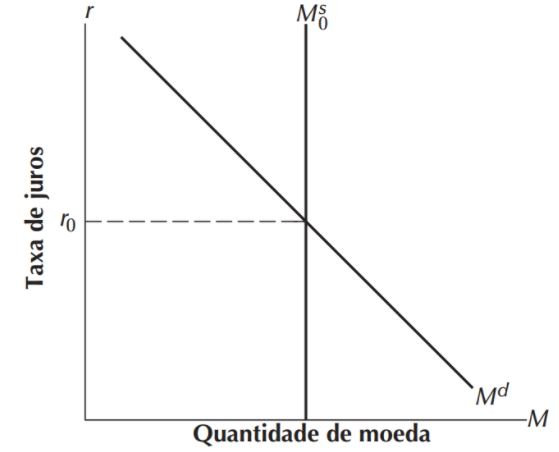
\includegraphics[width=0.5\textwidth]{./figures/aula092_fig1.JPG}
    \caption{Determinação da taxa de juros de equilíbrio. Fonte: Froyen (2013).}
    \label{fig1}
\end{figure}
\end{frame}

\subsection{Teoria Keynesiana da demanda por moeda}
\begin{frame}{Teoria Keynesiana da demanda por moeda}
    \begin{itemize}
        \item A teoria Keynesiana da demanda por moeda considerava três motivos para reter moeda:
        \bigskip
        \begin{enumerate}
            \item \textcolor{blue}{Demanda por transações.} A moeda é um meio de troca e os indivíduos mantem moeda para uso em transações. A quantidade de moeda mantida para transações variaria positivamente com o volume de transações de que o indivíduo participasse.
            \bigskip
            \item \textcolor{blue}{Demanda precaucionária.} Além da moeda mantida para transações planejadas, saldos adicionais de moeda são mantidas para o gasto de gastos inesperados (e.g., despesas médicas ou consertos). Keynes acreditava que o montante mantido para esse fim dependia positivamente da renda.
            \bigskip
            \item \textcolor{blue}{Demanda especulativa.} Por que manter moeda acima da quantidade necessária para os motivos de transações e precaucionários, se títulos pagam juros e moeda não?
        \end{enumerate}
    \end{itemize}
\end{frame}

\begin{frame}{Teoria Keynesiana da demanda por moeda}
    \begin{itemize}
        \item Essa demanda adicional por moeda existe por causa da incerteza sobre as taxas de juros futuras e da relação entre mudanças na taxa de juros e preço dos títulos.
        \bigskip
        \item Se fosse esperado que as taxas de juros se movessem de modo a causar perdas de capital para os títulos, era possível que essas perdas esperadas superassem os ganhos de juros dos títulos e fizessem com que o investidor preferisse manter moeda.
        \bigskip
        \item Essa moeda seria mantida pelos que especulam em relação a mudanças futuras na taxa de juros.
        \bigskip
        \item Dada a relação inversa entre juros e preço dos títulos, uma elevação nas taxas de juros de mercado resulta em uma perda de capital para os títulos já existentes.
        \bigskip
        \item Uma queda na taxa de juros resulta em um ganho de capital para os títulos já existentes.
    \end{itemize}
\end{frame}

\begin{frame}{Teoria Keynesiana da demanda por moeda}
\begin{itemize}
    \item Os retornos esperados dos dois ativos podem ser expressos como se segue:
    \begin{eqnarray}
    \text{retorno da moeda } &=& 0 \nonumber \\
    \text{retorno esperado dos títulos } &=& i \begin{cases}
    (+) \text{ ganho de capital esperado} \\
    (-) \text{ perda de capital esperada}
    \end{cases} \nonumber
    \end{eqnarray}
    \bigskip
    \item O retorno sobre a moeda é igual a zero pois, como estamos assumindo, este ativo não rende nenhum tipo de juros e, além disso, seu valor não é sujeito a ganhos ou perdas de capital à medida que a taxa de juros varia.
    \bigskip
    \item Note que, então, não estamos permitindo efeitos que variações nos preços de mercadorias tem sobre a moeda.
    \bigskip
    \item O valor \textcolor{purple}{real} da moeda declina proporcionalmente com aumentos no nível de preços agregado.
    \bigskip
    \item No entanto, o mesmo acontece com o valor real dos títulos e, portanto, os retornos relativos não são diretamente afetados por variações nos preços dos bens.
\end{itemize}
\end{frame}

\begin{frame}{Teoria Keynesiana da demanda por moeda}
    \begin{itemize}
        \item Os títulos irão pagar uma taxa de juros igual a $i$.
        \bigskip
        \item O retorno \textcolor{purple}{esperado} dos títulos será igual à taxa de juros somado ou subtraído dos ganhos ou perdas esperados de capital.
        \bigskip
        \item Como discutimos anteriormente, um investidor que espera uma queda na taxa de juros antecipa um ganho de capital, enquanto um investidor que antecipa um aumento na taxa de juros espera uma perda de capital.
        \bigskip
        \item Essa incerteza com relação ao futuro das taxas de juros é crucial para a análise de Keynes.
    \end{itemize}
\end{frame}

\begin{frame}{Teoria Keynesiana da demanda por moeda}
    \begin{itemize}
        \item Suponha um investidor que espera uma redução futura na taxa de juros.
        \bigskip
        \item Os títulos, então, teriam um retorno esperado maior. Além de pagar juros, espera-se um ganho de capital sobre esses títulos.
        \bigskip
        \item No entanto, se antecipamos um aumento futuro na taxa de juros, é possível que a perda de capital esperada mais que compense o pagamento de juros sobre os títulos.
        \bigskip
        \item Neste caso, o retorno esperado sobre os títulos seria negativo e, então, a moeda seria um ativo preferível.
        \bigskip
        \item A moeda retida no momento anterior a uma queda no preço dos títulos (i.e., um aumento esperado na taxa de juros) é a \textcolor{purple}{demanda especulativa por moeda} de Keynes.
    \end{itemize}
\end{frame}

\begin{frame}{Teoria Keynesiana da demanda por moeda}
    \begin{itemize}
        \item Temos, então, uma relação entre quantidade de moeda demandada e as mudanças esperadas nas taxas de juros.
        \bigskip
        \item Keynes converte isso em uma relação entre a demanda por moeda e o \textcolor{blue}{nível} da taxa de juros por meio de um pressuposto sobre como as pessoas formam expectativas quanto a mudanças futuras na taxa de juros.
    \end{itemize}
\end{frame}

\begin{frame}{Teoria Keynesiana da demanda por moeda}
\begin{itemize}
    \item Pela teoria Keynesiana, o indivíduo tem uma noção preconcebida da taxa de juros natural, $r_i^n$.
    \bigskip
    \item A taxas de juros acima deste nível normal, espera-se que a taxa de juros caia, a essas taxas os títulos são preferíveis à moeda como ativo.
    \bigskip
    \item A demanda especulativa por moeda desse indivíduo ($M_i^2$) será zero e, portanto, a demanda por títulos será igual a $W_{hi} - M_i^1$ (onde $M_i^1$ é a demanda por motivos transação).
    \bigskip
    \item A demanda especulativa por moeda também será zero para taxas de juros pouco abaixo de $r_i^n$.
    \bigskip
    \item Isso porque se a taxa de juros não está muito abaixo de $r_i^n$, os ganhos com juros sobre títulos serão maiores que a perda de capital esperada.
    \bigskip
    \item A perda de capital esperada será pequena porque apenas uma pequena elevação na taxa de juros será esperada à medida que a taxa de juros $i$ retorna para $r_i^n$.
\end{itemize}
\end{frame}

\begin{frame}{Teoria Keynesiana da demanda por moeda}
\begin{itemize}
    \item Existe um valor de taxa de juros abaixo de $r_i^n$, no entanto, para o qual a perda esperada de capital sobre os títulos será igual aos ganhos de juros.
    \bigskip
    \item Chamamos este valor de \textcolor{purple}{taxa de juros crítica} do indivíduo ($r_i^c)$.
    \bigskip
    \item A qualquer taxa de juros acima da taxa crítica ($r_i^c$) a demanda especulativa individual por moeda é zero.
    \bigskip
    \item Abaixo da taxa de juros crítica, a moeda será preferida. O indivíduo troca títulos por moeda e, portanto, a demanda especulativa por moeda é igual a $M_{i}^{2} = W_{hi} - M_{i}^1$, o que significa que toda a riqueza dessa pessoa será mantida em moeda.
\end{itemize}
\end{frame}

\begin{frame}{Teoria Keynesiana da demanda por moeda}
    \begin{itemize}
        \item Keynes considerava que diferentes indivíduos tinham noções diferentes quanto ao que seria uma taxa de juros normal.
    \bigskip
    \item Conforme a taxa de juros caia a partir de uma taxa muito alta em que houvesse pouca demanda especulativa, ela desceria sucessivamente para níveis mais abaixo das taxas críticas de diferentes investidores.
    \bigskip
    \item Quanto mais baixa a taxa de juros, mais investidores julgariam que, dada a sua concepção da taxa de juros normal, a moeda seria o ativo preferível.
    \bigskip
    \item A uma taxa de juros muito baixa, quase todos os investidores esperariam uma elevação substancial da taxa de juros no futuro e a moeda seria quase unanimamente preferida como ativo.
    \bigskip
    \item Com isso podemos construir a demanda agregada por saldos especulativos de moeda.
    \end{itemize}
\end{frame}

\begin{frame}{Teoria Keynesiana da demanda por moeda}
\begin{figure}
    \centering
    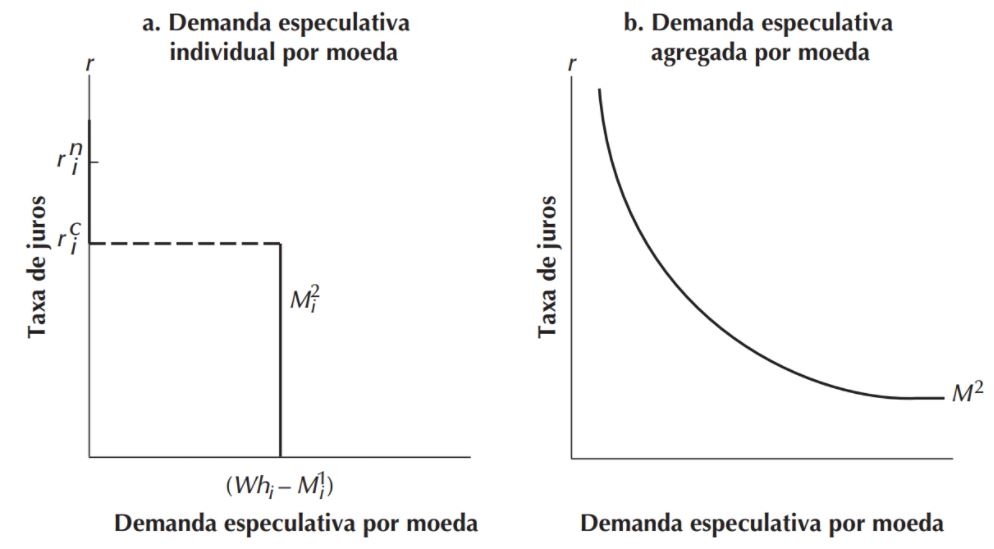
\includegraphics[width=0.8\textwidth]{./figures/aula092_fig2.JPG}
    \caption{Curvas de demanda especulativa individual e agregada por moeda. Fonte: Froyen (2013).}
    \label{fig2}
\end{figure}
\end{frame}

\begin{frame}{Teoria Keynesiana da demanda por moeda}
\begin{itemize}
    \item A Figura \ref{fig2} mostra que a curva de demanda especulativa agregada por moeda é suave, refletindo o aumento gradual da demanda agregada especulativa por moeda à taxas de juros sucessivamente mais baixas.
    \bigskip
    \item A curva vai ficando mais plana em uma taxa de juros muito baixa, o que mostra que, a essa taxa baixa, há uma expectativa geral de perdas de capital com os títulos que superam os ganhos com juros.
    \bigskip
    \item Nessa taxa, os incrementos à riqueza seriam mantidos em forma de moeda, sem queda adicional na taxa de juros.
    \bigskip
    \item \textcolor{blue}{Armadilha da liquidez:} situação em uma taxa de juros muito baixa em que a curva de demanda especulativa por moeda torna-se quase horizontal.
\end{itemize}
\end{frame}

\subsection{Demanda total por moeda}
\begin{frame}{Demanda total por moeda}
\begin{itemize}
    \item Podemos, agora, reunir os três motivos para reter moeda no sistema Keynesiano em uma função de demanda por moeda total.
    \bigskip
    \item A demanda para transações e precaucionária variam positivamente com a renda e negativamente com a taxa de juros. (Tobin e Baumol expandiram a análise de Keynes e mostraram que as taxas de juros influenciam também as demandas por transações e por motivos precaucionários).
    \bigskip
    \item A demanda especulativa por moeda está negativamente relacionada à taxa de juros.
    \bigskip
    \item Portanto, podemos expressar a demanda total por moeda como:
    \begin{equation}
        M^d = L(\$ Y, i), \qquad L'(Y) > 0, L'(i) < 0.
    \end{equation}
    \bigskip
    \item Reescrevendo a equação anterior como uma relação entre moeda real, renda real e taxa de juros, temos:
    \begin{equation}
        \frac{M^d}{P} = L(Y,i).
    \end{equation}
\end{itemize}
\end{frame}

\section{O modelo IS-LM tradicional}
\subsection{Derivação da curva LM}
\begin{frame}{Derivação da curva LM}
    \begin{figure}
        \centering
        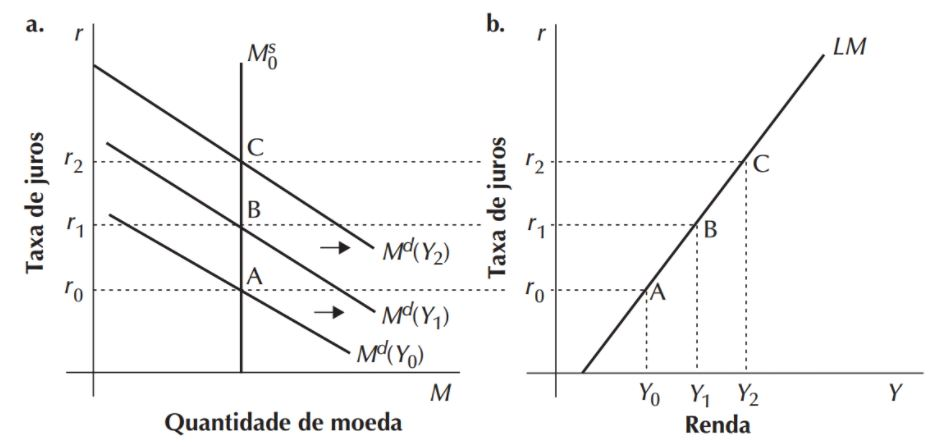
\includegraphics[width=0.9\textwidth]{./figures/aula092_fig3.JPG}
        \caption{Equilíbrio no mercado monetário e curva LM. Fonte: Froyen (2013).}
        \label{fig3}
    \end{figure}
\end{frame}

\subsection{Modelo IS-LM tradicional}
\begin{frame}{Modelo IS-LM tradicional}
    \begin{itemize}
        \item No modelo keynesiano tradicional, a variável de política monetária é a quantidade de moeda em circulação.
        \bigskip
        \item O modelo IS-LM tradicional pode, portanto, ser descrito pelas seguintes condições de equilíbrio simultâneo nos mercados de bens e monetário:
        \begin{eqnarray}
            Y &=& C(Y-T) + I(Y,i) + G, \\
            \frac{M}{P} &=& L(Y,i).
        \end{eqnarray}
    \end{itemize}
\end{frame}

\subsection{Exercícios}
\begin{frame}[t]{Exercício 1}
    Considere o modelo IS-LM para uma economia fechada, representado pelas seguintes equações:
    \begin{eqnarray*}
    C &=& 400 + 0,5Y_d, \\
    I &=& 300 - 600r, \\
    T &=& 100 + 0,2Y, \\
    G &=& 250, \\
    \frac{M^d}{P} &=& 2Y - 4000r, \\
    \frac{M^s}{P} &=& 600,
    \end{eqnarray*}
    em que $C$ é o consumo agregado, $Y_d$ a renda disponível, $I$ o investimento agregado, $r$ a taxa real de juros, $T$ o total de impostos pagos, $G$ o gasto do governo, $M^d$ a demanda por moeda nominal, $M^s$ a oferta de moeda nominal, $P$ o nível de preços, que é fixo. Não há transferências do governo para os consumidores.
\end{frame}

\begin{frame}[t]{Exercício 1}
Com base nessas informações, julgue as afirmativas:
\bigskip
\begin{enumerate}
    \item A poupança privada de equilíbrio é igual a 100.
    \bigskip
    \item O produto de equilíbrio é igual a 1100.
    \bigskip
    \item A taxa de juros real de equilíbrio é igual a 0,5.
    \bigskip
    \item Se a oferta de moeda aumentar em 100\%, com tudo o mais permanecendo constante, o produto de equilíbrio irá aumentar para 1200.
    \bigskip
    \item Se a alíquota de imposto direto for reduzida para zero, com tudo o mais mantido constante, o produto de equilíbrio irá expandir 20\%.
\end{enumerate}
\end{frame}

\begin{frame}[t]{Exercício 2}
Considere uma economia fechada, descrita pelas seguintes relações:
\begin{eqnarray*}
C &=& 20 + 0,25Y_d, \\
I &=& 10 + 0,25Y - 100r, \\
G &=& 20, \\
T &=& 20, \\
\frac{M^d}{P} &=& 2Y - 800r, \\
\frac{M^s}{P} &=& 120.
\end{eqnarray*}
Utilizando o instrumental IS-LM, determine o produto de equilíbrio.
\end{frame}

\begin{frame}{Modelo IS-LM tradicional}
    \begin{itemize}
        \item O modelo IS-LM tradicional determina os valores da renda agregada e taxa de juros que equilibram, de maneira simultânea, o mercado de bens e os mercados financeiros.
        \bigskip
        \item Como vimos anteriormente, o equilíbrio no mercado monetário implica equilíbrio no mercado de títulos. Portanto, teremos uma situação de equilíbrio em todos os três mercados.
        \bigskip
        \item O modelo IS-LM tradicional pode, portanto, ser descrito pelas seguintes condições de equilíbrio simultâneo nos mercados de bens e monetários:
        \begin{align}
            Y &= C(Y-T) + I(Y,i) + G, \tag{IS}\\
            \frac{M}{P} &= L(Y,i). \tag{LM}
        \end{align}
    \end{itemize}
\end{frame}

\subsection{Equilíbrio nos mercados financeiros: a relação LM}
\begin{frame}{Equilíbrio nos mercados financeiros: a relação LM}
    \begin{itemize}
        \item A demanda por moeda, no sistema Keynesiano, depende positivamente da renda agregada dados os motivos de transação e precaução.
        \bigskip
        \item A demanda por moeda relaciona-se negativamente com a taxa de juros devido ao motivo especulação e porque a quantidade de moeda retida por motivos transacionais a qualquer nível de renda declina à medida com que a taxa de juros aumenta (dado que o custo de oportunidade de reter esses balanços também aumenta).
        \bigskip
        \item O equilíbrio nos mercados financeiros, como vimos, é expresso pela seguinte relação:
        \[
        \frac{M}{P} = L(Y,i).
        \]
    \end{itemize}
\end{frame}

\begin{frame}{Equilíbrio nos mercados financeiros: a relação LM}
\begin{itemize}
    \item Podemos calcular a inclinação da curva LM tomando o diferencial total de primeira ordem da expressão anterior:
    \[
    \frac{1}{P}dM -\frac{M}{P^2}dP = L_YdY + L_idi.
    \]
    \bigskip
    \item Fazendo as variações das variáveis exógenas iguais a zero, obtemos a inclinação da curva LM:
    \[
    \frac{di}{dY} = -\frac{L_Y}{L_i} > 0.
    \]
\end{itemize}
\end{frame}

\begin{frame}{Equilíbrio nos mercados financeiros: a relação LM}
\begin{itemize}
    \item A curva LM é positivamente inclinada - a níveis mais elevados de renda, o equilíbrio nos mercados financeiros ocorre a taxas de juros mais altas.
    \bigskip
    \item Um aumento na renda agregada aumenta a quantidade demandada de moeda para uma dada taxa de juros, já que os motivos transacionais e precaucionários de demanda por moeda variam positivamente com a renda.
    \bigskip
    \item Quanto mais sensível for a curva de demanda por moeda às variações na renda, $L_Y$, mais inclinada será a curva LM. Neste caso, uma dada mudança na renda tem um efeito maior sobre a taxa de juros quanto mais elástica for a curva LM com relação à renda.
\end{itemize}
\end{frame}

\begin{frame}{Equilíbrio nos mercados financeiros: a relação LM}
\begin{itemize}
    \item Por outro lado, quanto menos sensível for a curva de demanda por moeda às variações na taxa de juros, maior a inclinação da curva LM.
    \bigskip
    \item Portanto, quanto menor a elasticidade-juros da demanda por moeda, menor o impacto que grandes mudanças na taxa de juros tem sobre o nível de demanda por moeda.
\end{itemize}
\end{frame}

\begin{frame}{Equilíbrio nos mercados financeiros: a relação LM}
\begin{figure}
    \centering
    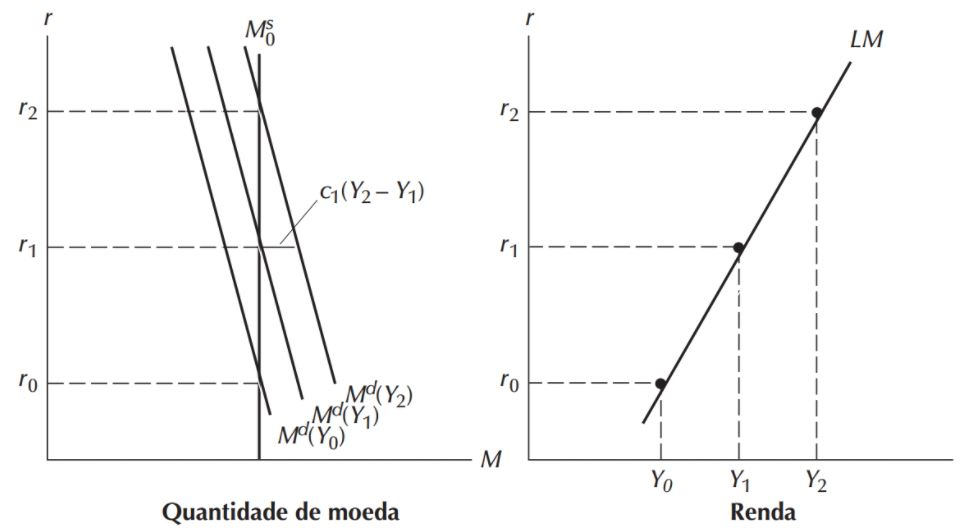
\includegraphics[width=0.8\textwidth]{./figures/aula092_fig4.JPG}
    \caption{Baixa elasticidade-juros da demanda por moeda. Fonte: Froyen (2013).}
    \label{fig4}
\end{figure}
\end{frame}

\begin{frame}{Equilíbrio nos mercados financeiros: a relação LM}
\begin{figure}
    \centering
    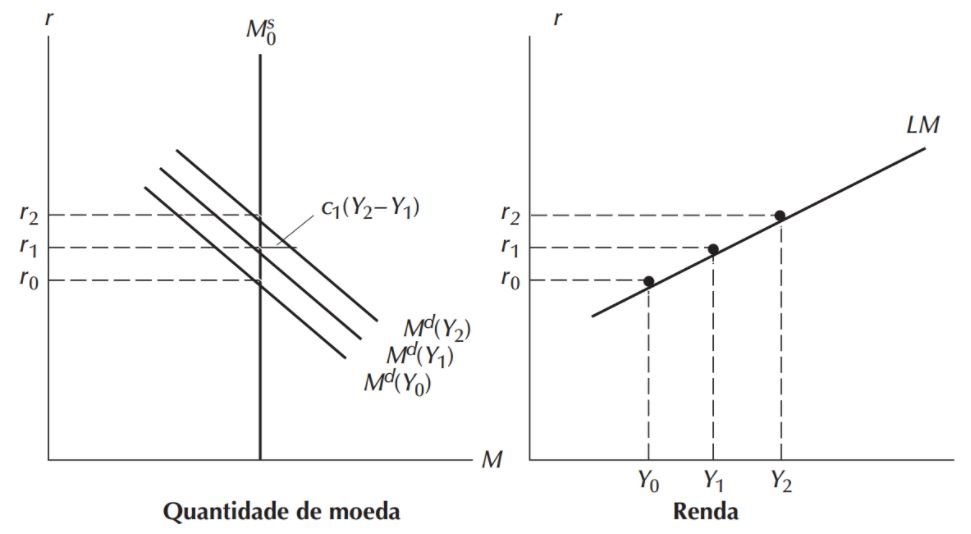
\includegraphics[width=0.8\textwidth]{./figures/aula092_fig5.JPG}
    \caption{Alta elasticidade-juros da demanda por moeda. Fonte: Froyen (2013).}
    \label{fig5}
\end{figure}
\end{frame}

\begin{frame}{Equilíbrio nos mercados financeiros: a relação LM}
\begin{itemize}
    \item Podemos observar dois casos extremos em nossa análise da inclinação da curva LM:
    \bigskip
    \begin{enumerate}
        \item Demanda por moeda completamente insensível a variações na taxa de juros. Nos referimos a este caso como o \textcolor{blue}{caso clássico}, já que a função de demanda por moeda Keynesiana não difere muito da demanda clássica - demanda por moeda depende apenas da renda.
        \bigskip
        \item Se a demanda por moeda for bastante sensível à taxa de juros, a curva LM ficará próxima à horizontal. Neste caso, uma pequena alteração na taxa de juros deve ser acompanhada de uma grande mudança no nível de renda, a fim de manter o equilíbrio no mercado monetário - \textcolor{blue}{armadilha da liquidez}.
    \end{enumerate}
\end{itemize}
\end{frame}

\begin{frame}{Equilíbrio nos mercados financeiros: a relação LM}
\begin{figure}
    \centering
    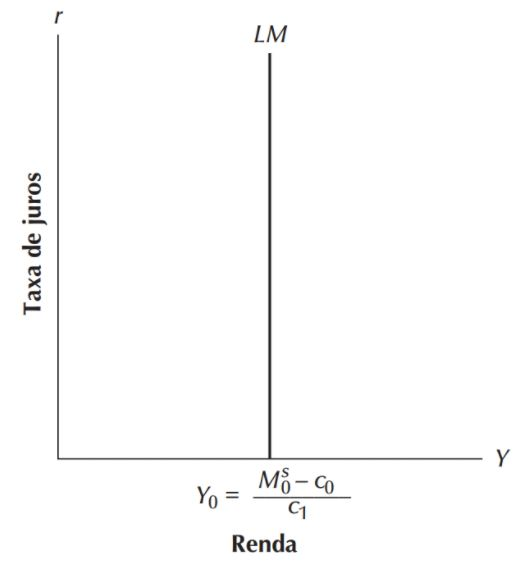
\includegraphics[width=0.4\textwidth]{./figures/aula092_fig6.JPG}
    \caption{Curva LM - caso clássico. Fonte: Froyen (2013).}
    \label{fig6}
\end{figure}
\end{frame}

\begin{frame}{Equilíbrio nos mercados financeiros: a relação LM}
\begin{figure}
    \centering
    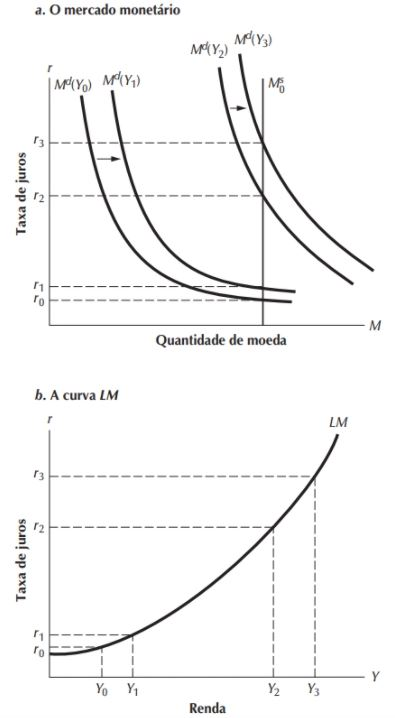
\includegraphics[width=0.25\textwidth]{./figures/aula092_fig7.JPG}
    \caption{Armadilha da liquidez. Fonte: Froyen (2013).}
    \label{fig7}
\end{figure}
\end{frame}

\begin{frame}{Equilíbrio nos mercados financeiros: a relação LM}
\begin{itemize}
    \item Em resumo, temos os seguintes principais pontos sobre a curva LM:
    \bigskip
    \begin{enumerate}
        \item É o conjunto de combinações de taxas de juros e níveis de renda que equilibram o mercado monetário.
        \bigskip
        \item É positivamente inclinada. Dada a oferta de moeda fixa, um aumento no nível de renda, que eleva a quantidade de moeda demandada, tem de ser seguido por uma aumento nas taxas de juros. Isso reduz a quantidade de moeda demandada e, portanto, mantém o equilíbrio no mercado monetário.
        \bigskip
        \item É mais inclinada quando a demanda por moeda responde fortemente à renda e fracamente às taxas de juros.
        \bigskip
        \item É deslocada por mudanças na oferta de moeda. Um aumento na oferta de moeda desloca a curva LM para a direita.
    \end{enumerate}
\end{itemize}
\end{frame}

\subsection{Equilíbrio no mercado de bens: relação IS}
\begin{frame}{Equilíbrio no mercado de bens: relação IS}
    \begin{itemize}
        \item Como a relação IS mantem-se a mesma, temos a mesma expressão para inclinação da curva IS:
        \begin{equation}
            \frac{di}{dY} = \frac{1-C_{Y_D}-I_Y}{I_i} \lessgtr 0.
        \end{equation}
        \bigskip
        \item Em resumo, temos os seguintes principais pontos sobre a curva IS:
        \bigskip
        \begin{enumerate}
            \item A curva IS é o conjunto de combinações de taxas de juros e níveis de renda que equilibram o mercado de bens.
            \bigskip
            \item A curva IS é negativamente inclinada porque um aumento na taxa de juros reduz o gasto com investimento planejado e, portanto, reduz demanda agregada diminuindo, assim, o nível de equilíbrio da renda.
            \bigskip
            \item Quanto menor for o multiplicador e menos sensível for o gasto com investimento em relação às variações na taxa de juros, mais inclinada será a curva IS.
            \bigskip
            \item A curva IS é deslocada por mudanças nos gastos autônomos. Um aumento nesses gastos (gastos governamentais ou queda nos impostos) desloca a curva IS para a direita.
        \end{enumerate}
    \end{itemize}
\end{frame}

\subsection{Equilíbrio nos mercados de bens e monetário}
\begin{frame}{Equilíbrio nos mercados de bens e monetário}
    \begin{figure}
        \centering
        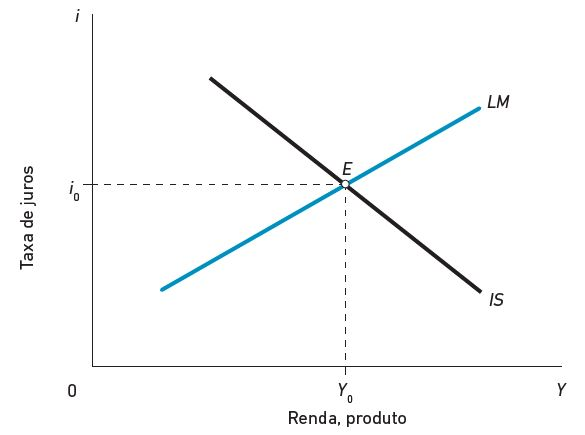
\includegraphics[width=0.6\textwidth]{./figures/aula092_fig8.JPG}
        \caption{Equilíbrio no mercado de bens e monetário. Fonte: Dornbusch, Fischer e Startz (2013).}
        \label{fig8}
    \end{figure}
\end{frame}

\begin{frame}{Equilíbrio nos mercados de bens e monetário}
\begin{itemize}
    \item A Figura \ref{fig8} resume nossa análise: a taxa de juros e o nível de produto agregado são determinados pela interação entre o mercado monetário (LM) e o mercado de bens (IS).
    \bigskip
    \item Os principais pressupostos em nossa análise é de que o nível de preços é constante e as firmas estão dispostas a fornecer qualquer quantidade de produto que for demandada naquele nível de preços.
    \bigskip
    \item Esse pressuposto é temporariamente necessário para fazermos nossa análise de curto prazo: ele corresponde ao pressuposto de uma curva de oferta agregada de curto prazo horizontal.
\end{itemize}
\end{frame}

\begin{frame}{Equilíbrio nos mercados de bens e monetário}
\begin{itemize}
    \item Os níveis de renda e da taxa de juros de equilíbrio variam quando a curva IS ou a curva LM se deslocam.
    \bigskip
    \item Consideremos, por exemplo, um aumento na taxa de investimento autônoma sobre os níveis de equilíbrio da renda e da taxa de juros.
    \bigskip
    \item Esse aumento eleva o gasto autônomo e, portanto, desloca a curva IS para a direita. Isso resulta em um aumento do nível da renda e da taxa de juros no ponto $E'$.
\end{itemize}
\end{frame}

\begin{frame}{Equilíbrio nos mercados de bens e monetário}
\begin{figure}
    \centering
    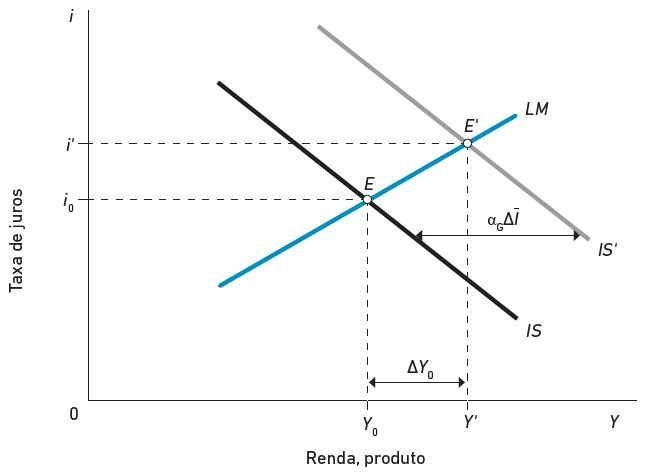
\includegraphics[width=0.6\textwidth]{./figures/aula092_fig9.JPG}
    \caption{Efeitos de um aumento no gasto autônomo. Fonte: Dornbusch, Fischer e Startz (2013).}
    \label{fig9}
\end{figure}
\end{frame}

\begin{frame}{Equilíbrio nos mercados de bens e monetário}
\begin{itemize}
    \item Se considerássemos apenas o mercado de bens, $\alpha_G\Delta\bar{I}$ seria a alteração no nível de renda resultante da variação no gasto autônomo de $\Delta\bar{I}$.
    \bigskip
    \item Mas pela Figura \ref{fig9} observamos que o aumento efetivo da renda agregada é de apenas $\Delta Y_0$ que é, claramente, menor que o deslocamento da curva IS.
    \bigskip
    \item Se a curva LM fosse horizontal, não haveria distinção entre a extensão do deslocamento da curva IS e a variação da renda e a taxa de juros não seria alterada quando a curva IS se deslocasse.
    \bigskip
    \item Qual a lógica econômica por trás? O aumento no gasto autônomo tende a elevar o nível de renda.
    \bigskip
    \item Um aumento da renda eleva a demanda por moeda. Como a oferta de moeda é fixa, a taxa de juros deve subir para garantir que a demanda por moeda permaneça igual à oferta.
    \bigskip
    \item Quando a taxa de juros sobe, os gastos com investimento reduzem. Consequentemente, a mudança do equilíbrio na renda é menor que o deslocamento da curva IS.    
\end{itemize}
\end{frame}

\section{Bibliografia}
\begin{frame}{\emoji{books} Bibliografia}
    \begin{itemize}
        \item BLANCHARD, O. Macroeconomia. 7.ed. São Paulo: Pearson Education do Brasil, 2017\medskip        
        \item DORNBUSCH, R.; FISCHER, S.; STARTZ, R. Macroeconomia. 11.ed. Porto Alegre: AMGH, 2013. Disponível em: \href{https://app.minhabiblioteca.com.br/books/9788580551853}{app.minhabiblioteca.com.br/books/9788580551853}\medskip
        \item FROYEN, R. Macroeconomia: teorias e aplicações. 2.ed. São Paulo: Saraiva, 2013. Disponível em: \href{https://app.minhabiblioteca.com.br/books/9788502175235}{app.minhabiblioteca.com.br/books/9788502175235}\medskip        
    \end{itemize}
\end{frame}
\end{document}